\documentclass[10pt,handout,english]{beamer}
\usetheme{Warsaw}
\usepackage{graphicx}
\usepackage{placeins}
\usepackage{amsmath, amssymb}
\usepackage{tabu}
\usepackage{bbm}
\usepackage{booktabs}
\usepackage[round]{natbib}
\usepackage{bm}
\usepackage{ragged2e}
\usepackage{bbm}
\usepackage{hyperref}
\usepackage{amsmath}
\usepackage{xcolor}
\usepackage[super]{nth}
\hypersetup{
    colorlinks=true,
    linkcolor=blue,
    filecolor=blue,      
    urlcolor=blue,
    citecolor=black,
}

\apptocmd{\frame}{}{\justifying}{} % Allow optional arguments after frame.

\setbeamertemplate{frametitle continuation}{}

\newcommand\setItemnumber[1]{\setcounter{enumi}{\numexpr#1-1\relax}}

\DeclareMathOperator{\tr}{tr}

\newcommand{\ts}{\textsuperscript}
\newcommand{\E}{\mathbb{E}}
\newcommand{\R}{\mathbb{R}}
\newcommand{\F}{\mathcal{F}}
\newcommand{\T}{\mathbb{T}}
\newcommand{\C}{\mathbb{C}}


\newcommand{\vertiii}[1]{{\left\vert\kern-0.25ex\left\vert\kern-0.25ex\left\vert #1 
    \right\vert\kern-0.25ex\right\vert\kern-0.25ex\right\vert}}


\title[]{Recovery in the noiseless setting}
\author[Kaveh S. Nobari]{Kaveh S. Nobari}
\institute[]{Lectures in High-Dimensional Statistics}
\date[27/10/2020]
{Department of Mathematics and Statistics\\ Lancaster University}
	

\begin{document}
\begin{frame}
\titlepage
\end{frame}


\begin{frame}{Contents}
\tableofcontents
\end{frame}

\section{Recovery in noiseless setting}

\begin{frame}[allowframebreaks]
To build intuition, we start with the simplest case, where the observations are \textcolor{red}{noiseless}. Essentially, we wish to find a solution $\theta$ to the linear system
\[
y=X\theta,
\]
where $y\in\R^n$ and $X\in\R^{n\times d}$, such that $d>n$. When $d>n$, this is an \textcolor{red}{undetermined} set of linear equations, so there is a whole subspace of solutions. 
{\vskip 0.5em}
If we have a \textcolor{red}{sparse solution} that means that there is a vector $\theta^*\in\R^d$, with at most $s\ll d$ non-zero entries and such that $y=X\theta^*$.
{\vskip 0.5em}
The goal is to find this sparse solution to the linear system.
\end{frame}

\subsection{$l_1$-based relaxation}
\frame{\tableofcontents[currentsection,currentsubsection]}

\begin{frame}[allowframebreaks]
This problem can be expressed as  a non-convex optimization problem involving the $l_0$-\textquotedblleft norm\textquotedblright. 
{\vskip 0.5em}
\textbf{Question:} The $l_0$-norm has been put in quotation marks, as it is not considered a \underline{proper} norm. Why is that?
{\vskip 0.5em}
Let us define
\[
\lVert \theta\rVert_0:=\sum\limits_{j=1}^{d}\mathbbm{1}[\theta_j\neq 0]
\] 
where $\mathbbm{1}$ is an indicator function. Thus, the optimization problem is
\[
\min_{\theta\in\R^d}\lVert \theta\rVert_0\quad\text{such that}\quad X\theta=y
\]
Solving this leads to obtaining a solution to the linear equations that has the fewest number of non-zero entries. How can we solve the above optimization problem? The constraint set is simply a subspace, but the cost function is \textcolor{red}{non-differentiable} and \textcolor{red}{non-convex}.
\end{frame}
\begin{frame}[allowframebreaks]
\begin{block}{Algorithm for solving the $l_0$ optimization problem}
\begin{enumerate}
\item[1)]  For each subset $S\subset \{1,\cdots,d\}$, we form the matrix $X_{S}\in\R^{\lvert S\rvert}$, consisting of the columns of $X$ indexed by S.
\item[2)] Examine the linear system $y=X_S\theta$ to see whether it has a solution $\theta\in\R^{\lvert S\rvert}$.
\item[3)] Iterate over subsets in increasing cardinality, then the first solution found would be the sparsest solution.
\end{enumerate}
\end{block}

What would be the computational cost of this optimisation approach be? If the sparsest solution contained $s$ non-zero entries, then we would have to search over at least 
\[
\sum\limits_{j=1}^{s-1}\binom{d}{j}
\]
subsets before finding it.

The next solution is to replace $l_0$ with the \textcolor{red}{nearest convex member} of the $l_q$ family, namely the $l_1$ norm. 
\begin{definition}[Convex relaxation]
When a non-convex optimization problem is approximated by a convex programme.
\end{definition}
In this setting this leads to the optimization problem
\[
\min_{\theta\in\R^d}\lVert \theta\rVert_1\quad\text{such that}\quad X\theta=y.
\]
The constraint set is a subspace (hence convex), and the cost function is piecewise linear and thus convex as well. The $l_1$ optimisation problem is a linear programme, since any piecewise linear convex cost can always be reformulated as the maximum of a collection of linear functions. The above optimisation problem is referred to as \textcolor{red}{basis pursuit linear programme} [see \citet{chen1998application}].
\end{frame}


\subsection{Exact recovery and restricted null space}
\frame{\tableofcontents[currentsection,currentsubsection]}

\begin{frame}[allowframebreaks]
When is solving the basis pursuit problem
\[
\min_{\theta\in\R^d}\lVert \theta\rVert_1\quad\text{such that}\quad X\theta=y.
\]
equivalent to solving the $l_0$ problem below?
\[
\min_{\theta\in\R^d}\lVert \theta\rVert_0\quad\text{such that}\quad X\theta=y
\]
Suppose $\theta^*=\R^d$ such that $y=X\theta^*$. Moreover, the vector $\theta^*$ has the support $S\subset\{1,2,\cdots,d\}$, which means that $\theta^*_j=0$ for all $j\in S^C$.
{\vskip 0.5em}
The success of the basis pursuit should depend on how the nullspace of $X$ is related to this support, where by definition
\[
\text{null}(X):=\{\Delta\in\R^d\mid X\Delta=0\}.
\]
Since $X\theta^*=y$ by assumption, any vector of the form $\theta^*+\Delta$ for some $\Delta\in\text{null}(X)$ is feasible for the basis pursuit programme.
{\vskip 0.5em}
Now let us consider the tangent cone of the $l_{1}$-ball at $\theta^{*}$, given by
\[
\T(\theta^{*})=\{\Delta\in\R^{d}\mid\lVert\theta^{*}+t\Delta\rVert_{1}\leq\lVert\theta^{*}\rVert_{1}\quad\text{for some}{\quad}{t>0}\}
\]
\end{frame}

\begin{frame}
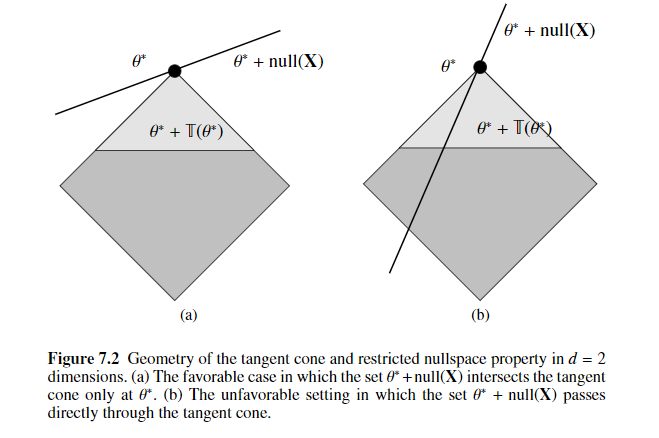
\includegraphics[width=\textwidth]{TangentCone.png}
\end{frame}

\begin{frame}[allowframebreaks]
\begin{itemize}
\setlength\itemsep{0.5em}
\item{} The set $\T(\theta^{*})$ captures the set of all directions relative to $\theta^{*}$ along which the $l_{1}$-norm remains constant or decreases. 
\item{} The solid line $\theta^{*}+\textnormal{null}(X)$ corresponds to the set of all vectors that are feasible for the basis pursuit linear programme, in the sense that $X(\theta^{*}+\text{null}(X))=y$.
\item{} In the above figures, if $\theta^{*}$ is optimal, then the tanget line $\theta^{*}+\text{null}(X)$ must only intersect with the tangent cone at $\theta^{*}$ implying that $\text{null}(X)$ at this point is zero vector.\justifying 
\item{} This intution leads to a condition on $X$, known as the \textcolor{red}{restricted nullspace property}.
\end{itemize}
\end{frame}
\begin{frame}[allowframebreaks]
 Let us define the cone subset
\[
\C(S)=\{\Delta\in\R^{d}\mid\lVert\Delta_{S^{c}}\rVert_{1}\leq\lVert\Delta_{S}\rVert_{1}\}
\]
which corresponds to the cone of vectors whose $l_{1}$-norm off the support (i.e. $S^{c}$), is dominated by the $l_{1}$-norm on the support (i.e. $S$). Using the defined cone subset, we can now formally define the restricted nullspace property
\begin{definition}[Restricted nullspace property]
The matrix $X$ is said to satisfy the restricted nullspace property with respect to $S$ if $\C(S)\cap\text{null}(X)={0}$.
\end{definition}
Let us now consider an alternative way of capturing the behavior of the tangent cone $\T(\theta^{*})$ that is independent of $\theta^{*}$, one which establishes that for any $S$-sparse vector $\theta^{*}$, the tangent cone $\T(\theta^{*})$ is contained within $\C(S)$, and conversely, that $\C(S)$ is contained in the union of such tangent cones.
{\vskip 0.5em}
More precisely, the restricted null space property is equivalent to the success of basis pursuit in the following sense:

\begin{theorem}
\begin{itemize}
\item[(a)] The matrix $X$ satisfies the restricted null space property with respect to $S$.
\item[(b)] For any vector $\theta^{*}\in\R^{d}$,with support $S$, the basis pursuit programme applied with $y=X\theta$ has a unique solution - i.e., $\hat{\theta}=\theta^{*}$.
\end{itemize}
\end{theorem}
{\vskip 0.5em}
\textbf{Proof:}

We begin by proving (a): since both $\hat{\theta}$ and $\theta^{*}$ are feasible for the basis pursuit programme, and since $\hat{\theta}$ is optimal, we have $\lVert\hat{\theta}\rVert_{1}\leq\lVert\theta^{*}\rVert_{1}$. Defining the error vector $\hat{\Delta}$ as follows
\[
\hat{\Delta}:=\hat{\theta}-\theta^{*}.
\]
By construction we have $X\theta^*=X\hat{\theta}=X(\theta^*+\hat{\Delta})$. From here we have
\begin{align*}
\lVert\theta_{S}^{*}\lVert_{1}=\lVert\theta^{*}\lVert_{1}&\geq\lVert \hat{\theta}\rVert_1\\
&\geq\lVert\theta^{*}+\hat{\Delta}\rVert_{1}\\
&=\lVert\theta^{*}+\hat{\Delta}_{S}+\hat{\Delta}_{S^{c}}\rVert_{1}\\
&=\lVert\theta_{S}^{*}+\underbrace{\theta_{S^c}^{*}}_{=0}+\hat{\Delta}_{S}\rVert_1+\lVert\hat{\Delta}_{S^{c}}\rVert_{1}
\end{align*}
From the triangle inequality, we know that
\[
\lVert\theta_{S}^{*}\rVert_{1}-\lVert\hat{\Delta}_{S}\rVert_{1}\leq\lVert\theta_{S}^{*}+\hat{\Delta}_{S}\rVert_{1}\leq\lVert\theta_{S}^{*}\rVert_1+\lVert\hat{\Delta}_{S}\rVert_{1}
\]
therefore
\begin{align*}
\lVert\theta_{S}^{*}\lVert_{1}=\lVert\theta^{*}\lVert_{1}&\geq\lVert\theta^{*}+\hat{\Delta}\rVert_{1}\\
&=\lVert\theta_{S}^{*}+\hat{\Delta}_{S}\rVert_{1}+\lVert\hat{\Delta}_{S^{c}}\rVert_{1}\\
&\geq\lVert\theta_{S}^{*}\rVert_{1}-\lVert\hat{\Delta}_{S}\rVert_{1}+\lVert\hat{\Delta}_{S^{c}}\rVert_{1}
\end{align*}
rearranging the above yields
\begin{align*}
\lVert\theta^{*}\rVert_{1}&\geq\lVert\theta_{S}^{*}\rVert_{1}-\lVert\hat{\Delta}_{S}\rVert_{1}+\lVert\hat{\Delta}_{S^{c}}\rVert_{1}\\
\lVert\theta^{*}\rVert_{1}-\lVert\theta_{S}^{*}\rVert_{1}&\geq-\lVert\hat{\Delta}_{S}\rVert_{1}+\lVert\hat{\Delta}_{S^{c}}\rVert_{1}\\
0&\geq-\lVert\hat{\Delta}_{S}\rVert_{1}+\lVert\hat{\Delta}_{S^{c}}\rVert_{1}\\
\lVert\hat{\Delta}_{S}\rVert_{1}&\geq	\lVert\hat{\Delta}_{S^{c}}\rVert_{1}
\end{align*}
which proves that $\hat{\Delta}\in\C(S)$. However, by construction, $X\hat{\Delta}=0$, which means that $\hat{\Delta}\in\text{null}(X)$ too. By the assumption imposed earlier, this implies that $\hat{\Delta}=0$ or that $\hat{\theta}=\theta^{*}$
\end{frame}
\begin{frame}
For (b) it suffices to show that, if the $l_1$ relaxation succeeds for all $S$-sparse vectors, then the set $\text{null}(X)\backslash\{0\}$ has no intersection with $\C(S)$.
{\vskip 0.5em}
For a given vector $\theta^*\in \text{null}(X)\backslash\{0\}$ consider the basis pursuit problem
\[
\min_{\beta\in\R^d}\lVert\beta\rVert_1,\quad \text{such that}\quad X\beta=X
\begin{bmatrix}
\theta_S*\\
0
\end{bmatrix}
\].
By assumption, the unique optimal solution will be $\hat{\beta}=(\theta_S^*,0 )'$. Since $X\theta^*=0$ by assumption, the vector $(0,-\theta_{S^c})'$ is also feasible for the problem, and, by uniqueness, we must have $\lVert\theta_S^*\rVert_1<\lVert\theta_{S^c}^*\rVert_1$, implying that $\theta\notin \C(S)$ as claimed.
\end{frame}

\subsection{Sufficient conditions for restricted null space}
\frame{\tableofcontents[currentsection,currentsubsection]}

\begin{frame}[allowframebreaks]
\begin{itemize}
\setlength\itemsep{0.5em}
\item{} To ensure that for any vector $\R^{d}$ with support $S$, the basis pursuit programme applied with $y=X\theta^{*}$ has unique solution $\hat{\theta}=\theta^{*}$, the matrix $X$ has to satisfy the restricted nullspace property. \justifying

\item{} The earliest sufficient conditions were based on the incoherence parameter of the design matrix, which is the quantity \justifying
\[
\delta_{pw}(X)=\max_{j,k=1,\cdots,d}\left\lvert\frac{\langle X_{j},X_{k}\rangle}{n}-\mathbbm{1}\{j=k\}\right\rvert
\]
where $X_{j}$ and $X_{k}$ are the $k\textsuperscript{th}$ and $j\textsuperscript{th}$ columns of the matrix $X$ respectively and $\mathbbm{1}\{.\}$ denotes an indicator function.  \justifying
\item{} $X$ is rescaled by dividing by $\sqrt{n}$, then $X_{j}'X_{j}=1$, which makes is more readily interpretable. The parameter $\delta_{pw}(X)$ essentially defines the maximum absolute value of cross-correlations between the columns of $X$.  \justifying
\end{itemize}
In what follows, through Exercise 7.3 of Wainright (2019), it will be shown that a small mutual (pairwise) incoherence is sufficient to guarantee a uniform version of the restricted nullspace property.

\begin{block}{Proposition}
If the pairwise incoherence satisfies the bound
\[
\delta_{pw}(X)\leq\frac{1}{3s}
\]
then the restricted nullspace property holds for all subsets $S$ of cardinality at most $s$.
\end{block}
\end{frame}
\begin{frame}[allowframebreaks]
\textbf{Proof:}
{\vskip 0.5em}
Choose a vector $\theta$ such that $X\theta=0$. For some set $S$ subject to $\vert S\vert\leq s$, we have $\theta=\theta_{S}+\theta_{S^{c}}$,and $X(\theta_{S}+\theta_{S^{c}})=0$. Thus, $X\theta_{S}=-X\theta_{S^{c}}$. Let us lower bound the $l_{2}$-norm of the left hand side of the former equation
\begin{align*}
\left\lVert\frac{X\theta_{S}}{\sqrt{n}}\right\Vert_{2}^{2}&=\frac{(X\theta_{S})'X\theta_{S}}{n}=\frac{\theta_{S}'X'X\theta_{S}}{n}\\
&=\frac{\theta_{S}'X'X\theta_{S}}{n}-\theta_{S}'\theta_{S}+\theta_{S}'\theta_{S}\\
&=\theta_{S}'\left(\frac{X'X}{n}-I\right)\theta_{S}+\text{\ensuremath{\Vert}\ensuremath{\theta_{S}\Vert_{2}^{2}}}
\end{align*}
since we have the inequality
\[
u'Mv\leq\vertiii{M}_{2}\lVert u\rVert_{1}\lVert v\rVert_{1}
\]
The term $\theta_{S}'\left(\frac{X'X}{n}-I\right)\theta_{S}$ can be expressed as follows 
\[
\theta_{S}'\left(\frac{X'X}{n}-I\right)\theta_{S}\leq\vertiii{\frac{X'X}{n}-I}_{2}\Vert\theta_{S}\Vert_{1}\Vert\theta_{S}\Vert_{1}
\]

Thus, 
\begin{align*}
\left\lVert\frac{X\theta_{S}}{\sqrt{n}}\right\rVert_{2}^{2}&=\theta_{S}'\left(\frac{X'X}{n}-I\right)\theta_{S}+\text{\ensuremath{\Vert}\ensuremath{\theta_{S}\Vert_{2}^{2}}}\\
&\geq-\vertiii{\frac{X'X}{n}-I}_{2}\Vert\theta_{S}\Vert_{1}^{2}+\ensuremath{\Vert}\ensuremath{\theta_{S}\Vert_{2}^{2}}
\end{align*}
since the mutual incoherence parameter is the smallest constant $\delta_{pw}(X)$ such that 
\[
\vertiii{\frac{X'X}{n}-I}_{2}\leq\delta_{pw}(X)
\]
we would thus have
\begin{align*}
\left\lVert\frac{X\theta_{S}}{\sqrt{n}}\right\rVert_{2}^{2}&=\theta_{S}'\left(\frac{X'X}{n}-I\right)\theta_{S}+\text{\ensuremath{\Vert}\ensuremath{\theta_{S}\Vert_{2}^{2}}}\\
&\geq-\vertiii{\frac{X'X}{n}-I}_{2}\Vert\theta_{S}\Vert_{1}^{2}+\ensuremath{\Vert}\ensuremath{\theta_{S}\Vert_{2}^{2}}\\
&\geq-\delta\lVert\theta_{S}\Vert_{1}^{2}+\lVert\theta_{S}\lVert_{2}^{2}
\end{align*}
Moreover, we have the inequality
\[
\lVert\theta_{S}\rVert_{1}\leq\sqrt{s}\lVert\theta_{S}\rVert_{2}
\]
which leads to
\begingroup
\allowdisplaybreaks 
\begin{align}
\left\lVert\frac{X\theta_{S}}{\sqrt{n}}\right\rVert_{2}^{2}&=\theta_{S}'\left(\frac{X'X}{n}-I\right)\theta_{S}+\text{\ensuremath{\Vert}\ensuremath{\theta_{S}\Vert_{2}^{2}}}\\
&\geq-\vertiii{\frac{X'X}{n}-I}_{2}\Vert\theta_{S}\Vert_{1}^{2}+\ensuremath{\Vert}\ensuremath{\theta_{S}\Vert_{2}^{2}}\\
&\geq-\delta\lVert\theta_{S}\Vert_{1}^{2}+\lVert\theta_{S}\lVert_{2}^{2}\\
&\geq-\delta s\lVert\theta_{S}\rVert_{2}^{2}+\lVert\theta_{S}\lVert_{2}^{2}=(1-\delta s)\lVert\theta_{S}\rVert_{2}^{2}
\end{align}
\endgroup
Since $X\theta_{S}=-X\theta_{S^{c}}$ we would also have 
\begingroup
\begin{align}
\allowdisplaybreaks
\left\lVert\frac{X\theta_{S}}{\sqrt{n}}\right\rVert_{2}^{2}&=\left\lvert\left\langle\frac{X\theta_S}{\sqrt{n}},\frac{-X\theta_{S^c}}{\sqrt{n}}\right\rangle\right\rvert\\
&=\left\lvert\theta_{S}'\left(\frac{X'X}{n}-I\right)\theta_{S}+\underbrace{\theta_{S}'\theta_{S^{c}}}_{=0}\right\rvert\\
&\leq\delta\lVert\theta_{S}\rVert_{1}\lVert\theta_{S^{c}}\rVert_{1}\\
&\leq\delta\sqrt{s}\lVert\theta_{S}\rVert_{2}\lVert\theta_{S^{c}}\rVert_{1}
\end{align}
\endgroup
Relating equations (1) and (5), we have 
\[
(1-\delta s)\lVert\theta_{S}\rVert_{2}^{2}\leq\left\lVert\frac{X\theta_{S}}{\sqrt{n}}\right\rVert_{2}^{2}\leq\delta\sqrt{s}\lVert\theta_{S}\rVert_{2}\lVert\theta_{S^{c}}\rVert_{1}
\]
Hence, we may write the above as
\begin{align}
(1-\delta s)\lVert\theta_{S}\rVert_{2}^{2}&\leq\delta\sqrt{s}\lVert\theta_{S}\rVert_{2}\lVert\theta_{S^{c}}\rVert_{1}\\
\lVert\theta_{S}\rVert_{2}^{2}&\leq\frac{\delta\sqrt{s}}{(1-\delta s)}\lVert\theta_{S}\rVert_{2}\lVert\theta_{S^{c}}\rVert_{1}
\end{align}
Recall the inequality $\lVert\theta_{S}\rVert_{1}\leq\sqrt{s}\lVert\theta_{S}\rVert_{2}$. Thus, multiplying equation (10) by $\sqrt{s}$, we will have
\begin{align*}
\sqrt{s}\lVert\theta_{S}\rVert_{2}^{2}&\leq\frac{s\delta}{(1-\delta s)}\lVert\theta_{S}\rVert_{2}\lVert\theta_{S^{c}}\rVert_{1}\\
\lVert\theta_{S}\rVert_{1}\leq\sqrt{s}\lVert\theta_{S}\rVert_{2}&\leq\frac{s\delta}{(1-\delta s)}\lVert\theta_{S}\rVert_{2}\lVert\theta_{S^{c}}\rVert_{1}\\
\lVert\theta_{S}\rVert_{1}\leq\sqrt{s}\lVert\theta_{S}\rVert_{2}&\leq\frac{s\delta}{(1-\delta s)}\lVert\theta_{S^{c}}\rVert_{1}\\
\end{align*}

Assuming $\delta\leq \frac{1}{2s}$, then $\lVert \theta_S\rVert_1\leq \lVert \theta_{S^c}\rVert_1$, therefore the restricted nullspace property holds. 

\end{frame}

\begin{frame}[allowframebreaks]
A more related but sophisticated sufficient condition is the \textcolor{red}{Restricted Isometry Property} (RIP). This can be understood as a generalisation of the pairwise incoherence condition, based on looking at conditioning of larger subsets of columns.

\begin{definition}[Restricted isometry property]

For a given integer $s\in\{1,\cdots,d\}$, we say that $X\in\R^{n\times d}$ satisfies the RIP of order $s$ with constant $\delta_{s}(X)>0$, if 
\[
\vertiii{\frac{X_{S}'X_{S}}{n}-I_{s}}_{2}\leq\delta_{s}(X)\quad\text{for all subests \ensuremath{S} of size at most \ensuremath{s}}
\]
\end{definition}

For $s=1$, we would have 
\begin{align*}
\vertiii{\frac{X_{j}'X_{j}}{n}-1}_{2}&\leq\delta_{1}\\
\left\lvert\frac{\lVert X_{j}\rVert_{2}^{2}}{n}-1\right\rvert&\leq\delta_{1}
\end{align*}
which implies 
\[
1-\delta_{1}\leq\frac{\lVert X_{j}\rVert_{2}^{2}}{n}\leq1+\delta_{1}
\]
for all $j=1,\cdots,d$. Now consider $s=2$, and suppose the matrix $X/\sqrt{n}$ has unit-norm columns. Then we would have
\[
\frac{X_{\{j,k\}}'X_{\{j,k\}}}{n}-\begin{bmatrix}1 & 0\\
0 & 1
\end{bmatrix}=\begin{bmatrix}\frac{\lVert X_{j}\rVert_{2}^{2}}{n}-1 & \frac{\langle X_{j,}X_{k}\rangle}{n}\\
\frac{\langle X_{j},X_{k}\rangle}{n} & \frac{\lVert X_{k}\rVert_{2}^{2}}{n}-1
\end{bmatrix}=\begin{bmatrix}0 & \frac{\langle X_{j,}X_{k}\rangle}{n}\\
\frac{\langle X_{j,}X_{k}\rangle}{n} & 0
\end{bmatrix}
\]

Now let us consider the $l_{2}$-matrix norm, which is the maximum singular value - i.e.,
\[
\vertiii{\frac{X_{\{j,k\}}'X_{\{j,k\}}}{n}-I_{2}}_{2}=\max_{j\neq k}\left\lvert\frac{\langle X_{j,}X_{k}\rangle}{n}\right\rvert=\delta_{pw}(X)
\]
\begin{definition}[Sandwich relation]

For any matrix $X$ and sparsity level $s\in{2,\cdots,d}$, we have the sandwich relation
\[
\delta_{pw}(X)\leq\delta_{s}(X)\leq s\delta_{pw}(X)
\]
and neither bound can be improved in general.

\end{definition}

Although RIP imposes constraints on much larger submatrices than pairwise incoherence, the magnitude of the constraints required to guarantee uniform RNS property can be milder. Suitable control on the RIP constants implies that the RNS property holds:

\begin{block}{Proposition}
If the RIP constant of order $2s$ is bounded as $\delta_{2s}(X)<1/2$, then the uniform RNS holds for any subset S of cardinality $\lvert S\rvert\leq s$.
\end{block}

Like pairwise incoherence constant, control on the RIP constants is sufficient condition for the BPLP to succeed. A major advantage of the RIP is that for various classes of random design matrices, it can be used to guarantee exactness of basis pursuit using a sample size n that is much smaller than that guaranteed by pairwise incoherence. The RIP approach overcomes the “quadratic barrier” - i.e., the requirement that the sample size n scales quadratically in the sparsity s, as in the pairwise incoherence approach.
\end{frame}

\begin{frame}[allowframebreaks]
\frametitle{References}
\bibliographystyle{apa}
\bibliography{References_HDStat}
\end{frame}

\end{document}